\chapter{Modelagem FrameWeb}
\label{sec-frameweb}
\vspace{-1cm}

\emph{\imprimirtitulo} é um sistema Web cuja arquitetura utiliza \textit{frameworks} comuns no desenvolvimento para esta plataforma. Desta forma, o sistema pode ser modelado utilizando a abordagem FrameWeb~\cite{souza-celebratingfalbo20}.

A Tabela~\ref{tabela-frameworks} indica os \textit{frameworks} presentes na arquitetura do sistema que se encaixam em cada uma das categorias de \textit{frameworks} que FrameWeb dá suporte. Em seguida, os modelos FrameWeb são apresentados para cada camada da arquitetura.

\begin{footnotesize}
	\begin{longtable}{|c|c|}
		\caption{\textit{Frameworks} da arquitetura do sistema separados por categoria.}
		\label{tabela-frameworks}\\\hline
		
		\rowcolor{lightgray}
		\textbf{Categoria de \textit{Framework}} & \textbf{\textit{Framework} Utilizado} \\\hline 
		\endfirsthead
		\hline
		\rowcolor{lightgray}
		\textbf{Categoria de \textit{Framework}} & \textbf{\textit{Framework} Utilizado} \\\hline 
		\endhead

		Controlador Frontal & Flask \\\hline

		Injeção de Dependências & Flask (Blueprints e extensões) \\\hline

		Mapeamento Objeto/Relacional & SQLAlchemy \\\hline

		Segurança & Flask Security \\\hline
	\end{longtable}
\end{footnotesize}

\section{Camada de Negócio}
\label{sec-frameweb-negocio}

\begin{figure}[H]
	\centering
	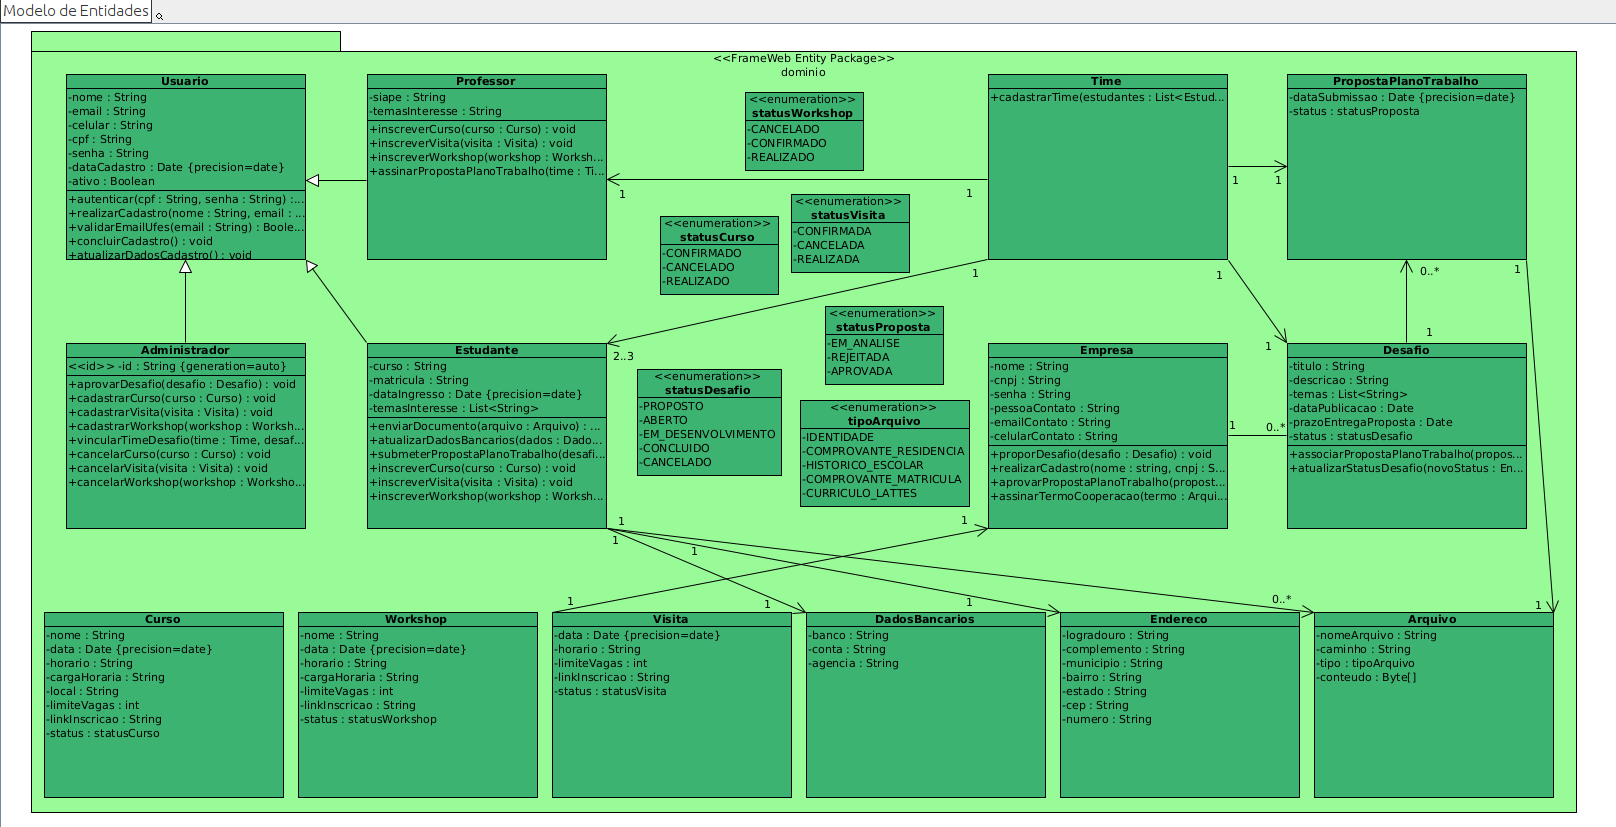
\includegraphics[width=1.0\textwidth]{figuras/figura_modelo_entidades.png}
	\caption{Modelo de entidades do FrameWeb.}
	\label{figura-entidades}
\end{figure}

\begin{figure}[H]
	\centering
	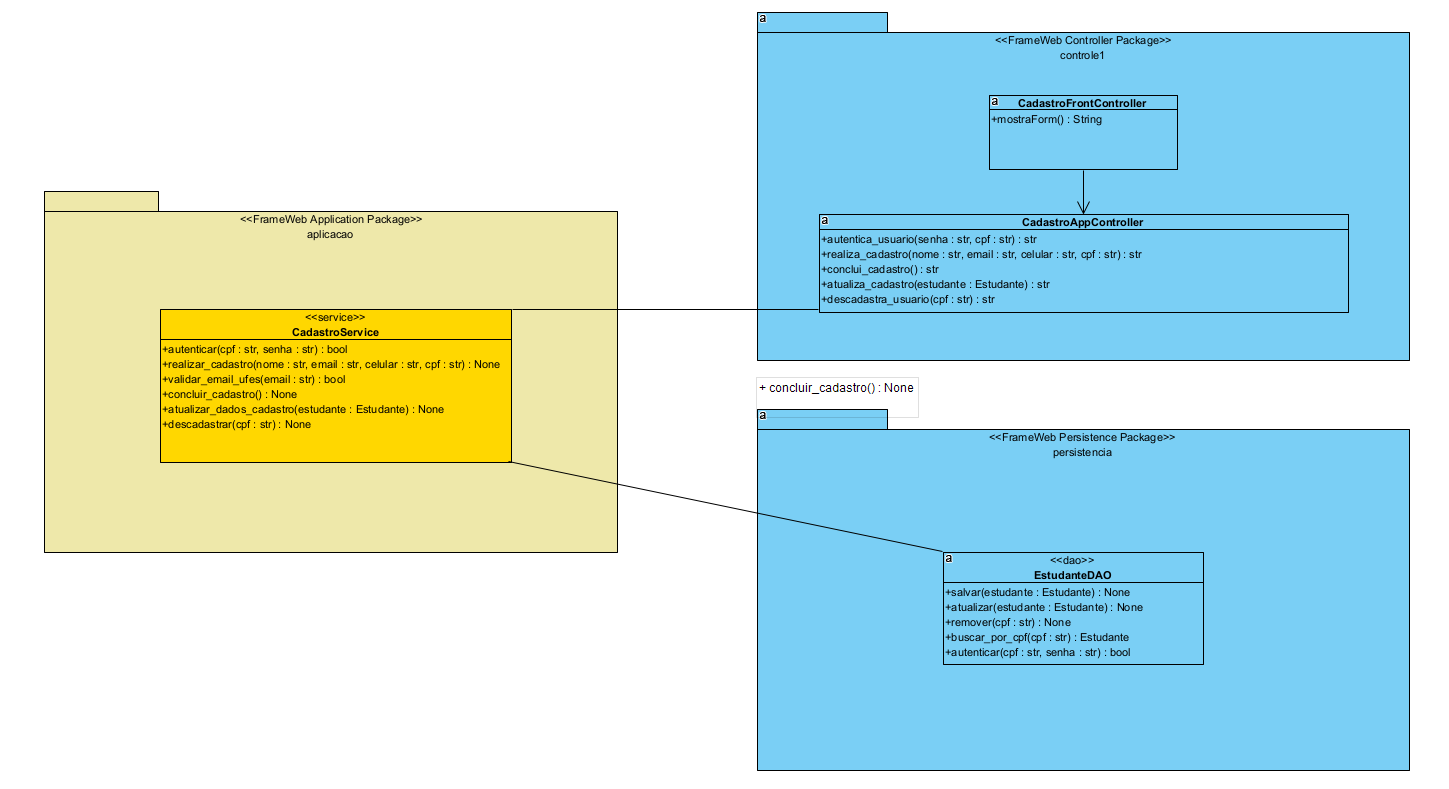
\includegraphics[width=1.0\textwidth]{figuras/figura_modelo_aplicacao.png}
	\caption{Modelo de aplicação do FrameWeb: Cadastro de Estudantes.}
	\label{figura-aplicacao}
\end{figure}

\section{Camada de Acesso a Dados}
\label{sec-frameweb-dados}

\begin{figure}[H]
	\centering
	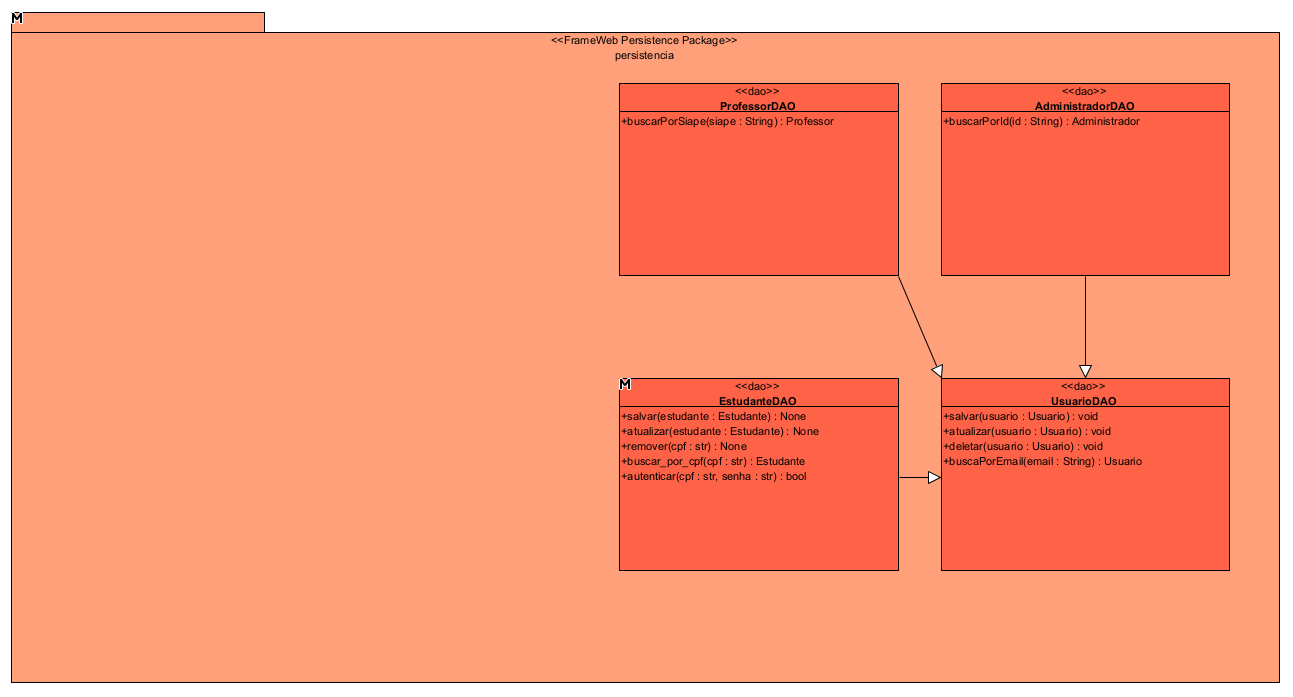
\includegraphics[width=1.0\textwidth]{figuras/figura_modelo_persistencia.png}
	\caption{Modelo de persistência do FrameWeb: Usuário.}
	\label{figura-persistencia}
\end{figure}

\section{Camada de Apresentação}
\label{sec-frameweb-apresentacao}

\begin{figure}[H]
	\centering
	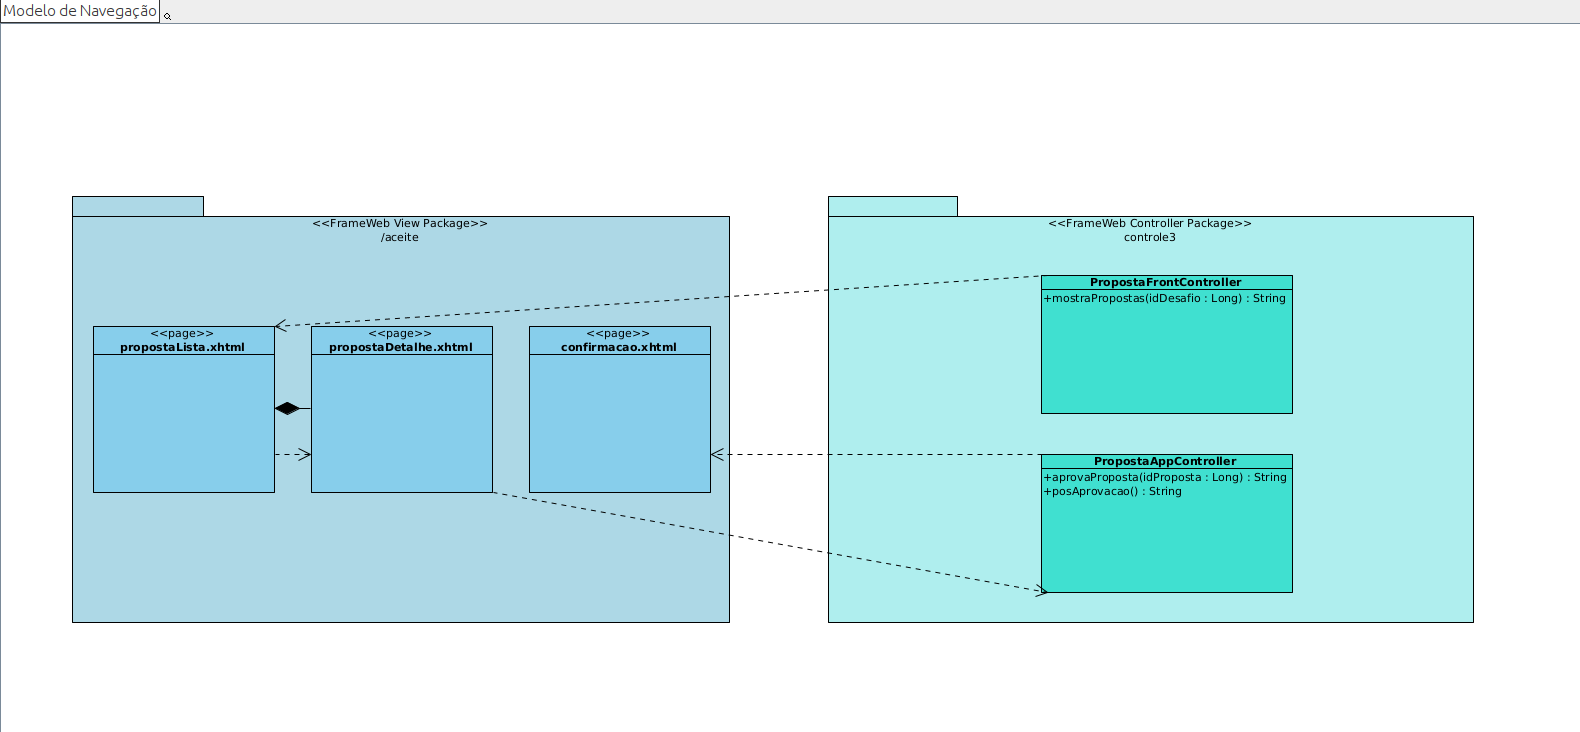
\includegraphics[width=1.0\textwidth]{figuras/figura_modelo_navegacao_cadastro.png}
	\caption{Modelo de navegação do FrameWeb - Cadastro.}
	\label{figura-cadastro}
\end{figure}

\begin{figure}[H]
	\centering
	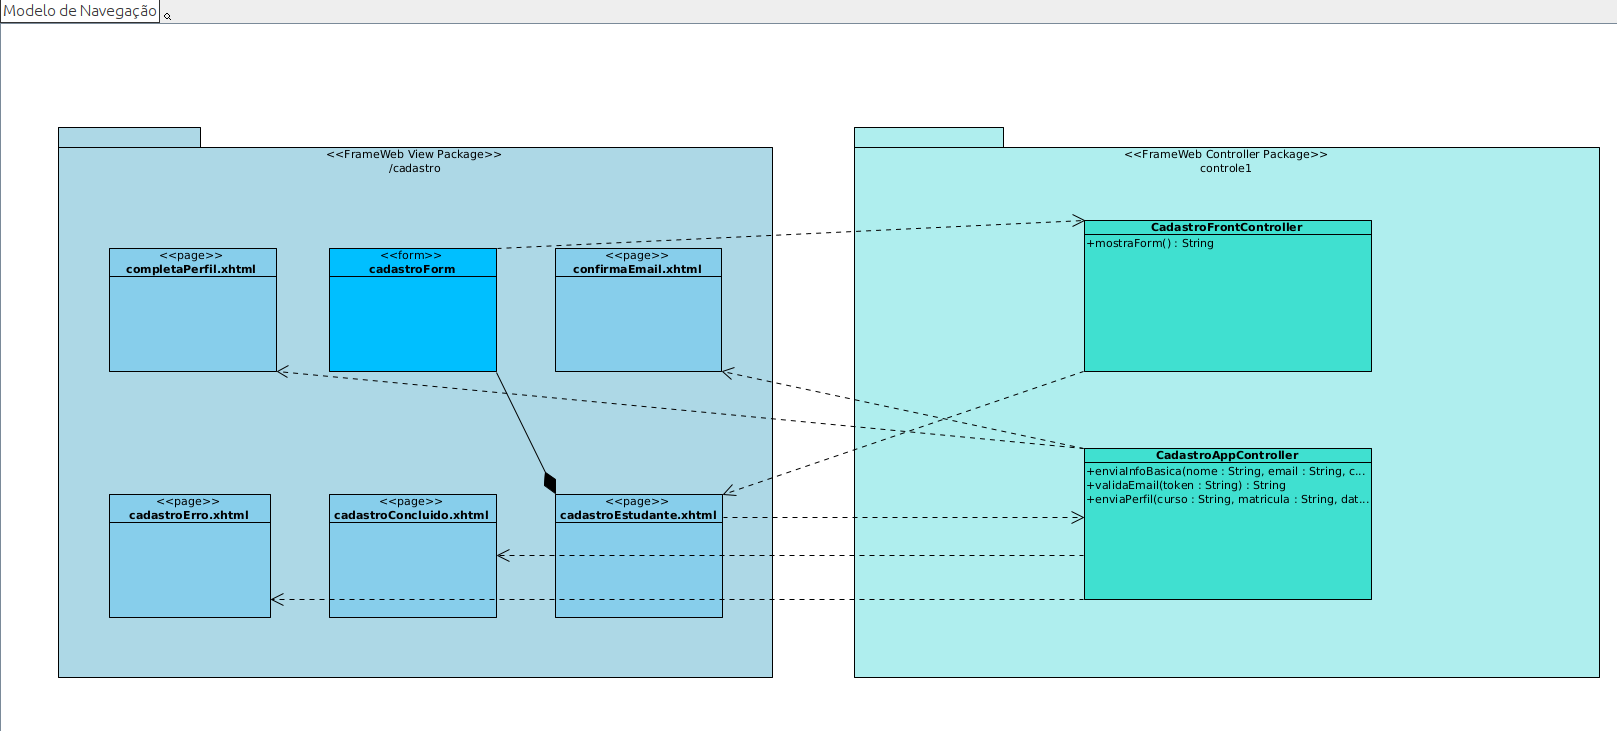
\includegraphics[width=1.0\textwidth]{figuras/figura_modelo_navegacao_notificacao.png}
	\caption{Modelo de navegação do FrameWeb - Notificação.}
	\label{figura-notificacao}
\end{figure}

\begin{figure}[H]
	\centering
	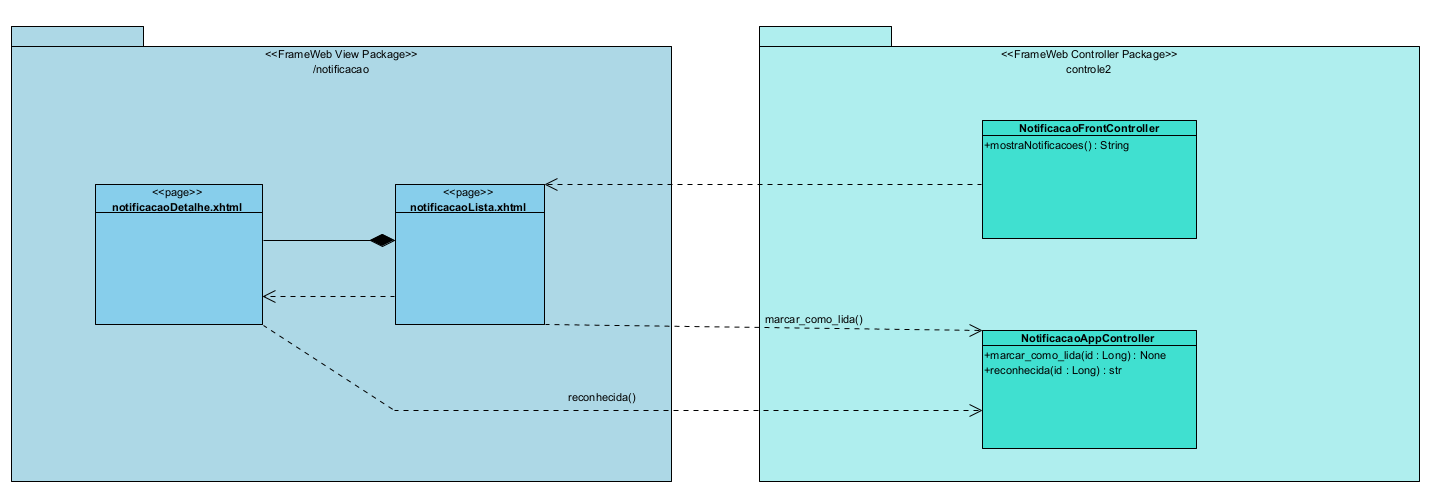
\includegraphics[width=1.0\textwidth]{figuras/figura_modelo_navegacao_aceite.png}
	\caption{Modelo de navegação do FrameWeb - Aceite.}
	\label{figura-aceite}
\end{figure}



